\documentclass[12pt,letterpaper]{article}
\usepackage[letterpaper,left=.78in,right=.78in,top=.69in,bottom=.70in]{geometry}
\usepackage{fontspec}
\usepackage{amsmath,unicode-math}
\usepackage{microtype}
\usepackage{xcolor,booktabs,array,tabularx}
\usepackage{tikz}
\usetikzlibrary{arrows.meta,positioning,calc}
\usepackage{hyperref}
\setmainfont{Latin Modern Roman}
\setsansfont{Latin Modern Sans}
\setmathfont{Latin Modern Math}
\definecolor{Ink}{HTML}{182D3A}
\definecolor{Deep}{HTML}{102B37}
\definecolor{Muted}{HTML}{405561}
\definecolor{Faint}{HTML}{B7C8CA}
\definecolor{Teal}{HTML}{006E63}
\definecolor{Blue}{HTML}{305F96}
\definecolor{Rust}{HTML}{9C482A}
\definecolor{Gold}{HTML}{F6C177}
\definecolor{TealTint}{HTML}{E8F3EF}
\definecolor{BlueTint}{HTML}{ECF1F8}
\definecolor{RustTint}{HTML}{F7ECE6}
\definecolor{Fog}{HTML}{F2F5F5}
\hypersetup{colorlinks,linkcolor=Teal,pdftitle={The Shape of Calculus},pdfsubject={Why these ten problems matter: an illustrated companion to Ten Problems That Teach Calculus},pdfdisplaydoctitle=true,bookmarksopen}
\setlength{\parindent}{0pt}
\setlength{\parskip}{4.5pt}
\setlength{\emergencystretch}{1.7em}
\setlength{\fboxsep}{0pt}
\linespread{1.07}
\pagestyle{empty}
\raggedbottom
\newcommand{\smallcap}[1]{{\sffamily\bfseries\fontsize{9}{11}\selectfont\addfontfeatures{LetterSpace=8}#1}}
\newcommand{\tagline}[1]{{\color{Accent}\smallcap{#1}}\par}
\newcommand{\headline}[1]{{\fontsize{38}{41}\selectfont\bfseries #1\par}}
\newcommand{\thinrule}{\noindent{\color{Faint}\rule{\linewidth}{.55pt}}\par}
\newcommand{\folio}[1]{\par\vfill\thinrule
  \noindent{\sffamily\small\color{Muted}The Shape of Calculus\enspace\textbar\enspace#1}
  \hfill{\sffamily\small\bfseries\color{Accent}\ifnum\value{page}<10 0\fi\thepage}\par}
\newcommand{\sectiontitle}[1]{\vspace{4pt}{\sffamily\bfseries\color{Accent}#1}\par\nobreak\vspace{-2pt}}
\newcommand{\chapter}[4]{\clearpage\colorlet{Accent}{#1}\pdfbookmark[1]{#2. #3}{c#2}
  \tagline{#2 \quad / \quad #4}\vspace{3pt}
  {\fontsize{31}{34}\selectfont\bfseries #3\par}\vspace{3pt}\thinrule}
\newcommand{\openq}[1]{\vspace{2pt}{\itshape\large\color{Muted}#1\par}\vspace{4pt}}
\newcommand{\plate}[2]{\par\noindent\colorbox{Fog}{\begin{minipage}{\linewidth}
  \vspace{7pt}\centering #1\par
  \end{minipage}}\par
  {\small\color{Muted}#2\par}\vspace{2pt}}
\newcommand{\bridge}[3]{\par\vspace{4pt}\noindent
  {\smallcap{\textcolor{Muted}{BUILD ON}}}\enspace#1
  \hfill{\smallcap{\textcolor{Accent}{THIS IDEA}}}\enspace#2
  \hfill{\smallcap{\textcolor{Muted}{NEXT}}}\enspace#3\par}
\newcommand{\tryit}[1]{\par\vspace{5pt}\noindent
 \colorbox{TealTint}{\begin{minipage}{\linewidth}
 \vspace{5pt}\hspace{10pt}\begin{minipage}{\dimexpr\linewidth-20pt\relax}
 {\smallcap{\textcolor{Teal}{TRANSFER TEST}}}\enspace #1
 \end{minipage}\vspace{6pt}
 \end{minipage}}\par}
\newcommand{\chaplink}[2]{\hyperlink{c#1.1}{#2}}
\newcommand{\uom}[1]{\,\mathrm{#1}}
\tikzset{axis/.style={draw=Muted,line width=.6pt,-{Latex[length=2mm]}},
 guide/.style={draw=Muted,densely dashed,line width=.55pt},
 fcurve/.style={draw=Teal,line width=1.15pt},
 bcurve/.style={draw=Blue,line width=1.05pt},
 rcurve/.style={draw=Rust,line width=1.05pt},
 lab/.style={font=\sffamily\small, text=Muted, inner sep=2pt},
 lead/.style={draw=Muted,-{Latex[length=1.65mm]},line width=.6pt},
 dot/.style={circle,fill=Teal,inner sep=1.65pt},
 card/.style={font=\sffamily\bfseries\small,align=center,minimum height=.46in,rounded corners=1.5pt,inner xsep=9pt}}
\begin{document}
\color{Ink}\colorlet{Accent}{Teal}
\pdfbookmark[0]{Start here}{start}
\tagline{A CONCEPTUAL COMPANION TO TEN PROBLEMS THAT TEACH CALCULUS}
\vspace{18pt}
{\fontsize{63}{61}\selectfont\bfseries The Shape\\of Calculus\par}
\vspace{11pt}
{\fontsize{22}{26}\selectfont\itshape\color{Muted}Why these ten problems matter\par}
\vspace{21pt}
\noindent\colorbox{Deep}{\begin{minipage}{\linewidth}
\vspace{16pt}
\centering
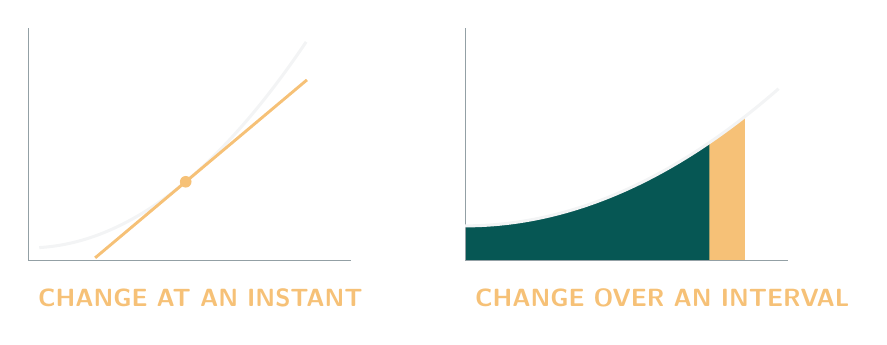
\begin{tikzpicture}[x=1cm,y=1cm]
\begin{scope}[shift={(0,0)}]
 \draw[white!55!Deep,thin] (0,0)--(4.1,0) (0,0)--(0,2.95);
 \draw[white!95!Deep,line width=1.1pt,domain=.14:3.53,samples=65] plot (\x,{.16+.21*\x*\x});
 \draw[Gold,line width=1.05pt] (.85,.034)--(3.54,2.294);
 \fill[Gold] (2.0,1.0) circle (2.1pt);
 \node[font=\sffamily\bfseries\small,text=Gold,anchor=west] at (0,-.48) {CHANGE AT AN INSTANT};
\end{scope}
\begin{scope}[shift={(5.55,0)}]
 \fill[Teal!65!Deep] (0,0)--plot[domain=0:3.55,samples=50] (\x,{.44+.11*\x*\x})--(3.55,0)--cycle;
 \fill[Gold] (3.10,0)--plot[domain=3.10:3.55,samples=18] (\x,{.44+.11*\x*\x})--(3.55,0)--cycle;
 \draw[white!55!Deep,thin] (0,0)--(4.1,0) (0,0)--(0,2.95);
 \draw[white!95!Deep,line width=1.1pt,domain=0:3.98,samples=65] plot (\x,{.44+.11*\x*\x});
 \node[font=\sffamily\bfseries\small,text=Gold,anchor=west] at (0,-.48) {CHANGE OVER AN INTERVAL};
\end{scope}
\end{tikzpicture}
\vspace{11pt}
\end{minipage}}
\vspace{17pt}

{\large You can learn to differentiate an expression without knowing when a derivative is the right tool. This reader starts with that decision. It asks what each problem makes visible, and how to recognize the same idea when the story changes.\par}
\vspace{10pt}
{\color{Teal}\smallcap{EXPERIENCE BEFORE EQUATION}}\par
Predict what will happen. Name the mathematical question. Then choose a formula, a graph, or a computation that can actually answer it.
\folio{Conceptual companion}

\clearpage\pdfbookmark[0]{A map of the course}{map}
\tagline{START HERE \quad / \quad READING MAP}
\vspace{4pt}\headline{A map of the course}
\vspace{4pt}
Limits give calculus a way to reason about processes we can begin but cannot literally finish. The derivative turns interval measurements into a local rate. The integral turns local contributions into a total. The Fundamental Theorem tells us how those two operations fit together.
\vspace{4pt}
\plate{
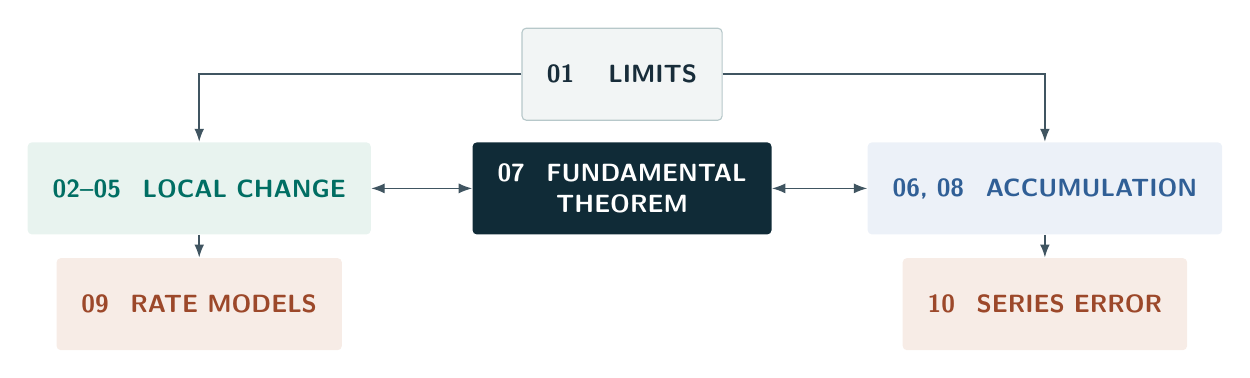
\begin{tikzpicture}[x=1cm,y=1cm]
\node[card,fill=Fog,draw=Faint,text=Ink] (L) at (7.1,3.25) {01 \quad LIMITS};
\node[card,fill=TealTint,text=Teal] (D) at (1.73,1.80) {02--05 \enspace LOCAL CHANGE};
\node[card,fill=BlueTint,text=Blue] (A) at (12.47,1.80) {06, 08 \enspace ACCUMULATION};
\node[card,fill=Deep,text=white] (F) at (7.1,1.80) {07 \enspace FUNDAMENTAL\\THEOREM};
\node[card,fill=RustTint,text=Rust] (O) at (1.73,.33) {09 \enspace RATE MODELS};
\node[card,fill=RustTint,text=Rust] (S) at (12.47,.33) {10 \enspace SERIES ERROR};
\draw[lead] (L.west) -| (D.north);
\draw[lead] (L.east) -| (A.north);
\draw[draw=Muted,{Latex[length=1.7mm]}-{Latex[length=1.7mm]}] (D.east)--(F.west);
\draw[draw=Muted,{Latex[length=1.7mm]}-{Latex[length=1.7mm]}] (F.east)--(A.west);
\draw[lead] (D.south)--(O.north);
\draw[lead] (A.south)--(S.north);
\end{tikzpicture}
}{The branching lines show major connections, not a strict prerequisite chain. Problem 10 also uses a definite integral to bound its series remainder.}

{\setlength{\tabcolsep}{6pt}\renewcommand\arraystretch{1.14}
\begin{tabularx}{\linewidth}{@{}lXr@{}}
\toprule
\smallcap{NO.}&\smallcap{QUESTION}&\smallcap{PAGE}\\
\midrule
01 & \chaplink{01}{Can an oscillation have a limit?} & 3\\
02 & \chaplink{02}{What happens at one instant?} & 4\\
03 & \chaplink{03}{How do linked things change?} & 5\\
04 & \chaplink{04}{Where is the best feasible choice?} & 6\\
05 & \chaplink{05}{How far can local knowledge go?} & 7\\
06 & \chaplink{06}{What do the changes add up to?} & 8\\
07 & \chaplink{07}{How fast is a total changing?} & 9\\
08 & \chaplink{08}{What if the interval never ends?} & 10\\
09 & \chaplink{09}{Can a rate law predict?} & 11\\
10 & \chaplink{10}{When can you stop adding terms?} & 12\\
\midrule
 & \hyperlink{toolkit.0}{The decision guide} \enspace / \enspace \hyperlink{key.0}{Transfer test notes} & 13--14\\
\bottomrule
\end{tabularx}}
\vspace{6pt}

{\small\color{Muted}\textbf{Use the three companions together.} Read this guide for the reason, the worked-solutions PDF for the derivation, and the numbered Python program for a plot or numerical check. Try each transfer question before looking at the notes on page 14.\par}
\folio{Reading map}

\chapter{Teal}{01}{Can an oscillation have a limit?}{FOUNDATIONS \quad LIMITS AND CONTINUITY}
\openq{Can a quantity keep reversing direction and still settle down?}
\plate{
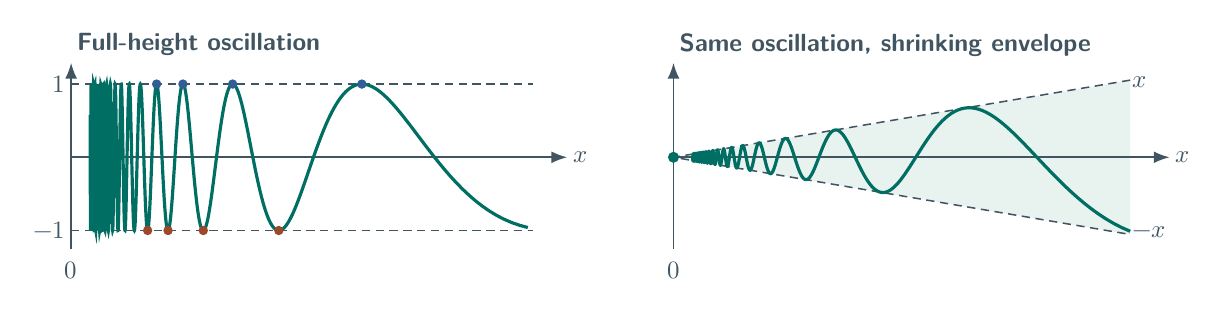
\begin{tikzpicture}[x=1cm,y=1cm]
\begin{scope}
\node[lab,anchor=west,font=\sffamily\bfseries\small] at (0,2.68) {Full-height oscillation};
\draw[axis] (0,1.25)--(6.30,1.25) node[lab,right] {\(x\)};
\draw[axis] (0,.09)--(0,2.45);
\draw[guide] (0,2.18)--(5.86,2.18) (0,.32)--(5.86,.32);
\draw[fcurve,domain=5:120,samples=1250] plot ({29/\x},{1.25+.93*sin(\x r)});
\foreach \n in {1,2,3,4}{
 \fill[Blue] ({29/(pi/2+2*pi*\n)},2.18) circle (1.7pt);
 \fill[Rust] ({29/(3*pi/2+2*pi*\n)},.32) circle (1.7pt);}
\node[lab,left] at (0,2.18) {\(1\)};
\node[lab,left] at (0,.32) {\(-1\)};
\node[lab,below] at (0,0) {\(0\)};
\end{scope}
\begin{scope}[shift={(7.65,0)}]
\node[lab,anchor=west,font=\sffamily\bfseries\small] at (0,2.68) {Same oscillation, shrinking envelope};
\fill[TealTint] (0,1.25)--(5.80,2.23)--(5.80,.27)--cycle;
\draw[guide] (5.80,2.23)--(0,1.25)--(5.80,.27);
\draw[axis] (0,1.25)--(6.30,1.25) node[lab,right] {\(x\)};
\draw[axis] (0,.09)--(0,2.45);
\draw[fcurve,domain=5:120,samples=1250] plot ({29/\x},{1.25+4.9/\x*sin(\x r)});
\fill[Teal] (0,1.25) circle (2pt);
\node[lab,right] at (5.75,2.20) {\(x\)};
\node[lab,right] at (5.75,.30) {\(-x\)};
\node[lab,below] at (0,0) {\(0\)};
\end{scope}
\end{tikzpicture}
}{Right-hand behavior of \(\sin(1/x)\) and \(x\sin(1/x)\). The blue and rust dots mark values of \(1\) and \(-1\). On the right, both sides of the envelope meet at zero. No finite plot can show every oscillation.}

\sectiontitle{Why this problem earned its place}
In many introductory exercises, substitution produces the right answer. That can leave you thinking a limit is a trick for plugging in a number. Here, both formulas are undefined at zero, and both oscillate faster as you approach it, yet only one has a limit. Because the examples differ by just a factor of \(x\), you can see what decides the matter. It's not whether the function keeps moving. It's whether its values are forced as close as you want to one number.

\sectiontitle{Where it sits in calculus}
This is the foundation for the rest of the course. Two sequences tending to the same input but giving incompatible outputs are enough to disprove a limit. A shrinking bound, such as \(\lvert x\sin(1/x)\rvert\leq\lvert x\rvert\), proves one even when the expression is hard to track. The same idea reappears when Taylor and series remainders are controlled in Problems 05 and 10.

\sectiontitle{What to notice in the Python}
The plot can show the two sequences and the shrinking envelope. It cannot inspect every point near zero. The proof comes from how the sequences are constructed and from a bound that holds for \emph{every} nonzero \(x\), not from how convincing the graph looks.

\bridge{Functions}{Limits by bounding}{Derivatives and sums}
\tryit{Without trying to graph it, find \(\lim_{x\to0}x^2\cos(1/x^3)\). Which part of the expression matters for your conclusion?}
\folio{Foundations}

\chapter{Teal}{02}{What happens at one instant?}{LOCAL CHANGE \quad THE DERIVATIVE}
\openq{A stopwatch measures a time interval. How can it help us find a speed at one instant?}
\plate{
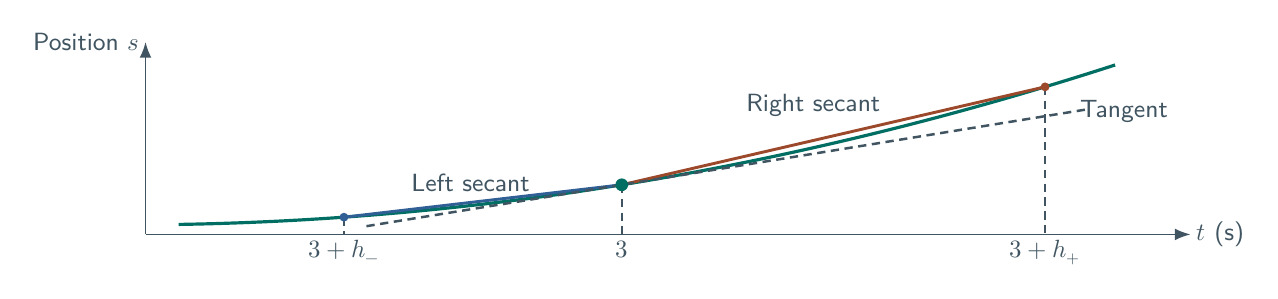
\begin{tikzpicture}[x=1.68cm,y=.235cm]
\draw[axis] (0,0)--(7.9,0) node[lab,right] {\(t\) (s)};
\draw[axis] (0,0)--(0,10.4) node[lab,left] {Position \(s\)};
\begin{scope}[shift={(0.25,0)}]
\draw[fcurve,domain=0:7.08,samples=80] plot (\x,{.54+.12*\x+.155*\x*\x});
\draw[guide] (1.25,.93)--(1.25,0) (3.35,2.68)--(3.35,0) (6.55,7.98)--(6.55,0);
\draw[bcurve] (1.25,.932)--(3.35,2.682);
\draw[rcurve] (3.35,2.682)--(6.55,7.975);
\draw[draw=Muted,densely dashed,line width=.9pt] (1.42,.446)--(6.86,6.75);
\fill[Teal] (3.35,2.682) circle (2.3pt);
\fill[Blue] (1.25,.932) circle (1.6pt);
\fill[Rust] (6.55,7.975) circle (1.6pt);
\node[lab,above left] at (2.7,1.99) {Left secant};
\node[lab,above left] at (5.35,6.02) {Right secant};
\node[lab,right] at (6.77,6.65) {Tangent};
\node[lab,below] at (3.35,0) {\(3\)};
\node[lab,below] at (1.25,0) {\(3+h_-\)};
\node[lab,below] at (6.55,0) {\(3+h_+\)};
\end{scope}
\end{tikzpicture}
}{Schematic of position versus time. Each secant uses two readings. Move both outside readings toward \(t=3\), and the two slopes tend to the tangent slope.}

\sectiontitle{Why this problem earned its place}
The cart has a simple position law, so the algebra doesn't compete with the main idea. An average velocity is available before you know any calculus. The problem asks you to shrink the interval on either side and notice that both averages go to the same number. The power rule would give the right result, \(6\uom{m/s}\), but it would skip the reason that number describes one instant.

\sectiontitle{Where it sits in calculus}
This is the definition from which differentiation rules get their meaning. Locally, a differentiable function behaves like a line, and the derivative is the slope of that line. That single idea later becomes a rate that can be related to other rates (03), a test for an interior optimum (04), and a first prediction of nearby behavior (05).

\sectiontitle{What to notice in the Python}
The program uses nonzero \(h\) in the original quotient and compares it with the simplified expression \(6+h\). For very tiny \(h\), subtracting nearly equal floating-point positions can actually make the computed quotient worse. The mathematically simpler expression also happens to be more numerically stable here.

\bridge{Limits}{Instantaneous rate}{Chain rule}
\tryit{A distance sensor provides one reading per second. How would you estimate velocity at a middle reading? What evidence would tell you whether a shorter interval improves your estimate?}
\folio{Local change}

\chapter{Teal}{03}{How do linked things change?}{LOCAL CHANGE \quad RELATED RATES}
\openq{If the ladder's foot moves at a steady speed, does its top have to move steadily too?}
\plate{
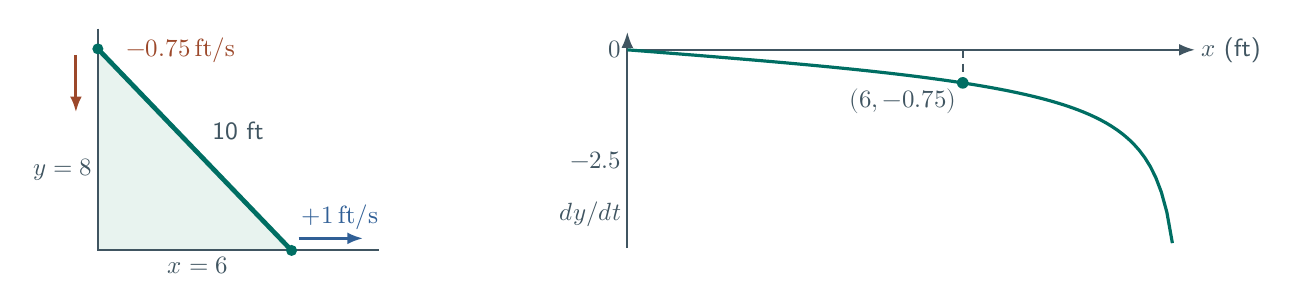
\begin{tikzpicture}[x=.41cm,y=.32cm]
\fill[TealTint] (0,0)--(6,0)--(0,8)--cycle;
\draw[draw=Muted,line width=.75pt] (0,8.8)--(0,0)--(8.7,0);
\draw[fcurve,line width=1.7pt] (0,8)--(6,0) node[pos=.52,above right=3pt,lab] {10 ft};
\draw[rcurve,-{Latex[length=2mm]}] (-.68,7.76)--(-.68,5.48);
\draw[bcurve,-{Latex[length=2mm]}] (6.22,.48)--(8.22,.48);
\fill[Teal] (0,8) circle (2pt) (6,0) circle (2pt);
\node[lab,left] at (0,3.2) {\(y=8\)};
\node[lab,below] at (3.1,0) {\(x=6\)};
\node[lab,anchor=west,text=Rust] at (.70,7.95) {\(-0.75\uom{ft/s}\)};
\node[lab,above,text=Blue] at (7.5,.57) {\(+1\uom{ft/s}\)};
\begin{scope}[shift={(16.4,0)},x=.71cm,y=.56cm]
\draw[axis] (0,4.55)--(10.15,4.55) node[lab,right] {\(x\) (ft)};
\draw[axis] (0,.05)--(0,4.95);
\draw[fcurve,domain=0:9.75,samples=100] plot (\x,{4.55-\x/sqrt(100-\x*\x)});
\draw[guide] (6,4.55)--(6,3.80);
\fill[Teal] (6,3.80) circle (2.1pt);
\node[lab,below left] at (6,3.80) {\((6,-0.75)\)};
\node[lab,left] at (0,4.55) {\(0\)};
\node[lab,left] at (0,2.05) {\(-2.5\)};
\node[lab,left] at (0,.83) {\(dy/dt\)};
\end{scope}
\end{tikzpicture}
}{The same fixed ladder permits many configurations and many speed ratios. The curve gives the top's vertical velocity for the same outward foot speed at different positions.}

\sectiontitle{Why this problem earned its place}
It separates \emph{how two quantities are related} from \emph{how fast they change}. You can picture one rigid triangle changing shape, but you can't infer equal endpoint speeds from a fixed ladder length. The speed ratio depends on the shape at that instant. The diagram lets you predict the sign and compare the speeds before differentiating.

\sectiontitle{Where it sits in calculus}
The chain rule applies even when neither quantity has been written explicitly as a function of time. In \(x^2+y^2=L^2\), both \(x\) and \(y\) are functions of \(t\). Differentiate that relationship first, then insert the snapshot values. If you insert \(x=6\) and \(y=8\) too early, the relationship becomes a number statement and the motion disappears. The same move returns for a changing integration limit in 07. With more variables, it leads to questions about how one change propagates through a system.

\sectiontitle{What to notice in the Python}
The program computes the top's velocity from the chain-rule formula, then checks it by moving the foot slightly forward and backward in time and recomputing the height. That second route uses geometry and a finite difference rather than the derived rate formula.

\bridge{Instantaneous rate}{Coupled rates}{Composed functions}
\tryit{The water level rises at the same speed in two tanks. One has straight sides and one widens toward the top. In which tank does maintaining that rise require a changing inflow rate, and why?}
\folio{Local change}

\chapter{Teal}{04}{Where is the best feasible choice?}{LOCAL CHANGE \quad OPTIMIZATION}
\openq{A tiny cut makes a shallow box. A very large cut leaves almost no base. Where do the two effects balance?}
\plate{
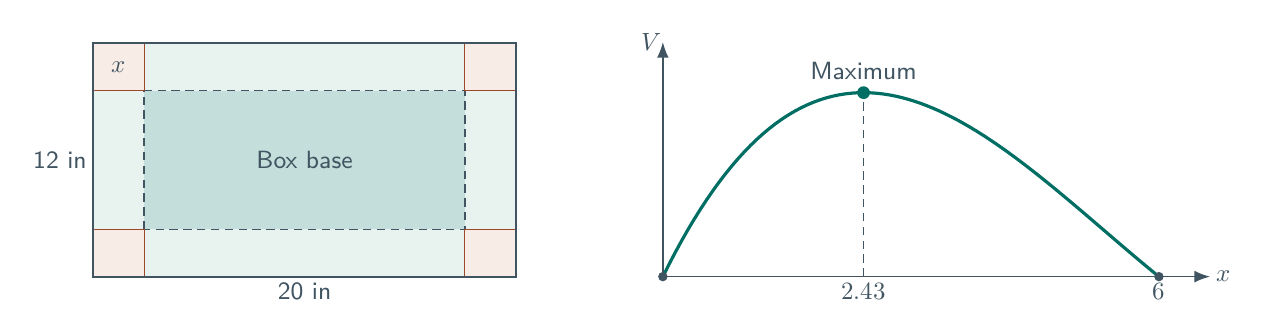
\begin{tikzpicture}[x=1cm,y=1cm]
\begin{scope}[x=.269cm,y=.247cm]
\fill[TealTint] (0,0) rectangle (20,12);
\fill[Teal!23!white] (2.43,2.43) rectangle (17.57,9.57);
\draw[guide] (2.43,2.43) rectangle (17.57,9.57);
\foreach \x in {0,17.57}{\foreach \y in {0,9.57}{\draw[draw=Rust,fill=RustTint] (\x,\y) rectangle ++(2.43,2.43);}}
\draw[draw=Muted,line width=.7pt] (0,0) rectangle (20,12);
\node[lab] at (10,6) {Box base};
\node[lab] at (1.22,10.78) {\(x\)};
\node[lab,below] at (10,0) {20 in};
\node[lab,left] at (0,6) {12 in};
\end{scope}
\begin{scope}[shift={(7.24,0)},x=1.05cm,y=.0089cm]
\draw[axis] (-.05,0)--(6.62,0) node[lab,right] {\(x\)};
\draw[axis] (0,0)--(0,335) node[lab,left] {\(V\)};
\draw[fcurve,domain=0:6,samples=80] plot (\x,{\x*(12-2*\x)*(20-2*\x)});
\draw[guide] (2.4274,0)--(2.4274,262.68);
\fill[Teal] (2.4274,262.68) circle (2.3pt);
\fill[Muted] (0,0) circle (1.7pt) (6,0) circle (1.7pt);
\node[lab,above] at (2.4274,272) {Maximum};
\node[lab,below] at (2.4274,0) {\(2.43\)};
\node[lab,below] at (6,0) {\(6\)};
\end{scope}
\end{tikzpicture}
}{The physical construction defines the domain before calculus begins. The other root of \(V'(x)=0\) is about \(8.24\) inches and does not belong on this plot of feasible cuts.}

\sectiontitle{Why this problem earned its place}
You can make the model out of a piece of paper and see the trade-off. Increasing the cut adds height while taking away base area. There is also a built-in trap. Algebra produces a stationary point that can't be built. The learner has to decide what a number means, not just calculate it.

\sectiontitle{Where it sits in calculus}
Optimization has three jobs. Specify the objective, determine the feasible domain, and justify the best candidate. A derivative finds stationary points in the interior, but endpoints and places where the derivative does not exist may also matter. Here the volume is smooth and the endpoints collapse the box. That leaves one feasible interior stationary point. Later, the same structure supports minimizing material, error, time, or cost, including in problems with several adjustable inputs.

\sectiontitle{What to notice in the Python}
The code treats roots as a list to filter, then evaluates the objective on the candidates that remain. A grid search is a useful independent check, but it can only say which \emph{sampled} cut was best. To turn the solution into a reusable method, preserve both the feasibility test and the candidate comparison.

\bridge{Derivative}{Best feasible choice}{Design trade-offs}
\tryit{You're asked to make the biggest box, but it must be no more than 2 inches deep. Which candidates now matter? Can you choose the winner without solving a new quadratic?}
\folio{Local change}

\chapter{Teal}{05}{How far can local knowledge go?}{LOCAL CHANGE \quad TAYLOR APPROXIMATION}
\openq{If you know a function's value, slope, and second derivative at one point, what can you promise about a nearby value?}
\plate{
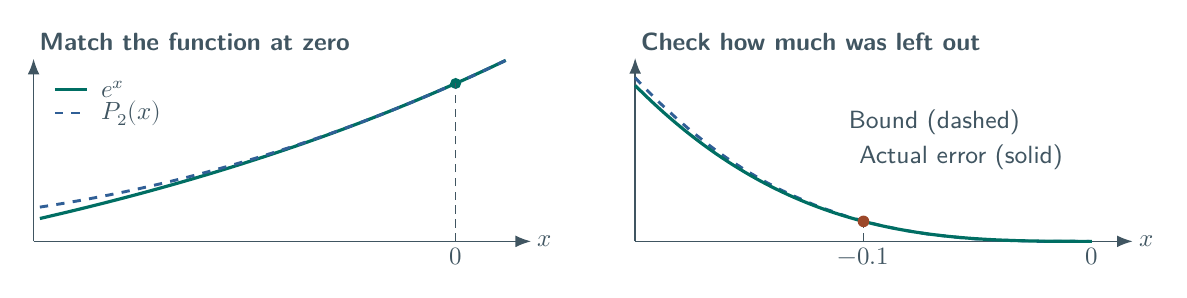
\begin{tikzpicture}[x=1cm,y=1cm]
\begin{scope}
\node[lab,anchor=west,font=\sffamily\bfseries\small] at (0,2.73) {Match the function at zero};
\draw[axis] (0,.20)--(6.32,.20) node[lab,right] {\(x\)};
\draw[axis] (0,.20)--(0,2.52);
\draw[fcurve,domain=-.66:.08,samples=75] plot ({8*(\x+.67)},{.43+3.55*(exp(\x)-.5)});
\draw[bcurve,dashed,domain=-.66:.08,samples=75] plot ({8*(\x+.67)},{.43+3.55*(1+\x+\x*\x/2-.5)});
\fill[Teal] (5.36,2.205) circle (2pt);
\draw[guide] (5.36,.20)--(5.36,2.205);
\node[lab,below] at (5.36,.2) {\(0\)};
\draw[fcurve] (.27,2.13)--(.68,2.13);
\node[lab,right] at (.78,2.13) {\(e^x\)};
\draw[bcurve,dashed] (.27,1.83)--(.68,1.83);
\node[lab,right] at (.78,1.83) {\(P_2(x)\)};
\end{scope}
\begin{scope}[shift={(7.64,0)}]
\node[lab,anchor=west,font=\sffamily\bfseries\small] at (0,2.73) {Check how much was left out};
\draw[axis] (0,.20)--(6.32,.20) node[lab,right] {\(x\)};
\draw[axis] (0,.20)--(0,2.53);
\draw[bcurve,dashed,domain=-.20:0,samples=80] plot ({29*(\x+.2)},{.20+1560*abs(\x*\x*\x)/6});
\draw[fcurve] plot coordinates {(0.000000,2.180025) (0.072500,2.107856) (0.145000,2.037433) (0.217500,1.968739) (0.290000,1.901751) (0.362500,1.836451) (0.435000,1.772817) (0.507500,1.710830) (0.580000,1.650470) (0.652500,1.591716) (0.725000,1.534548) (0.797500,1.478944) (0.870000,1.424886) (0.942500,1.372352) (1.015000,1.321322) (1.087500,1.271774) (1.160000,1.223689) (1.232500,1.177046) (1.305000,1.131823) (1.377500,1.088000) (1.450000,1.045557) (1.522500,1.004471) (1.595000,0.964723) (1.667500,0.926290) (1.740000,0.889153) (1.812500,0.853289) (1.885000,0.818678) (1.957500,0.785298) (2.030000,0.753128) (2.102500,0.722146) (2.175000,0.692332) (2.247500,0.663663) (2.320000,0.636119) (2.392500,0.609677) (2.465000,0.584316) (2.537500,0.560014) (2.610000,0.536749) (2.682500,0.514500) (2.755000,0.493245) (2.827500,0.472961) (2.900000,0.453628) (2.972500,0.435222) (3.045000,0.417722) (3.117500,0.401106) (3.190000,0.385351) (3.262500,0.370435) (3.335000,0.356336) (3.407500,0.343032) (3.480000,0.330500) (3.552500,0.318717) (3.625000,0.307661) (3.697500,0.297310) (3.770000,0.287641) (3.842500,0.278631) (3.915000,0.270257) (3.987500,0.262497) (4.060000,0.255328) (4.132500,0.248726) (4.205000,0.242669) (4.277500,0.237134) (4.350000,0.232098) (4.422500,0.227537) (4.495000,0.223428) (4.567500,0.219749) (4.640000,0.216475) (4.712500,0.213583) (4.785000,0.211051) (4.857500,0.208853) (4.930000,0.206968) (5.002500,0.205370) (5.075000,0.204037) (5.147500,0.202945) (5.220000,0.202070) (5.292500,0.201387) (5.365000,0.200874) (5.437500,0.200506) (5.510000,0.200259) (5.582500,0.200109) (5.655000,0.200032) (5.727500,0.200004) (5.800000,0.200000)};
\draw[guide] (2.9,.20)--(2.9,.455);
\fill[Rust] (2.9,.45363) circle (2.1pt);
\node[lab,below] at (2.9,.20) {\(-0.1\)};
\node[lab,below] at (5.8,.20) {\(0\)};
\node[lab] at (3.8,1.71) {Bound (dashed)};
\node[lab] at (4.14,1.27) {Actual error (solid)};
\end{scope}
\end{tikzpicture}
}{Agreement between the curves is hard to judge by eye near zero. A separate error plot makes the small difference visible. The bound is a guarantee, not a measurement of that difference.}

\sectiontitle{Why this problem earned its place}
The question isn't just whether you can replace an exponential by an easier expression. It's whether you can tell someone how far off the replacement could be. The example makes that distinction concrete. The quadratic gives \(0.905\), and Taylor's theorem says the error is less than \(0.000167\). You can decide whether the shortcut meets an accuracy requirement before looking up the exact function value.

\sectiontitle{Where it sits in calculus}
Differentiation first gives a local line. Taylor polynomials extend that local model by matching more derivatives. The first terms encode the value, slope, and bending near the reference point. The remainder tells you what is not captured. This is a bridge to numerical methods and power series, where knowing that a method works is different from knowing how much work is enough.

\sectiontitle{What to notice in the Python}
The program calculates its approximation without calling the exponential at the target. It then calls the library exponential to check the actual error and plots it against the bound. In a setting where the true value is unavailable, the guarantee still comes from the bound.

\bridge{Local linearity}{Approximation with error}{Series}
\tryit{You know the quadratic approximation is slightly high and at most \(0.000167\) high. Does that guarantee that \(0.905\) is correct to three decimal places? To four?}
\folio{Local change}

\chapter{Blue}{06}{What do the changes add up to?}{ACCUMULATION \quad THE DEFINITE INTEGRAL}
\openq{If the cart goes backward and then forward, how can it travel 2 meters but end up only \(\tfrac23\) meter from where it started?}
\plate{
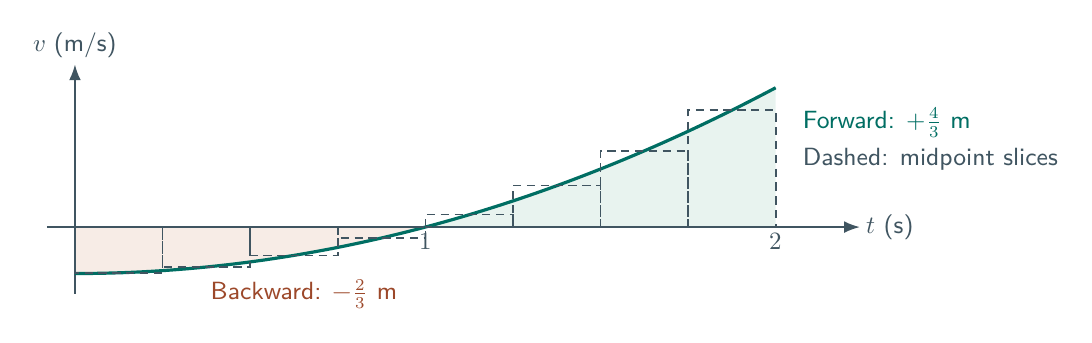
\begin{tikzpicture}[x=4.45cm,y=.59cm]
\fill[RustTint] (0,0)--plot[domain=0:1,samples=35] (\x,{\x*\x-1})--cycle;
\fill[TealTint] (1,0)--plot[domain=1:2,samples=35] (\x,{\x*\x-1})--(2,0)--cycle;
\draw[axis] (-.08,0)--(2.24,0) node[lab,right] {\(t\) (s)};
\draw[axis] (0,-1.43)--(0,3.5) node[lab,above] {\(v\) (m/s)};
\draw[fcurve,domain=0:2,samples=75] plot (\x,{\x*\x-1});
\foreach \i in {0,...,7}{
 \pgfmathsetmacro{\val}{((\i+.5)/4)^2-1}
 \draw[guide] ({\i/4},0) rectangle ++(.25,\val);}
\node[lab,below] at (1,0) {\(1\)};
\node[lab,below] at (2,0) {\(2\)};
\node[lab,text=Rust,anchor=west] at (.37,-1.44) {Backward: \(-\tfrac23\) m};
\node[lab,text=Teal,anchor=west] at (2.06,2.25) {Forward: \(+\tfrac43\) m};
\node[lab,anchor=west] at (2.06,1.45) {Dashed: midpoint slices};
\end{tikzpicture}
}{Each rectangle estimates a short change in position. Adding the rectangles with signs measures net change. Adding their magnitudes measures total travel.}

\sectiontitle{Why this problem earned its place}
A positive velocity for the whole trip would allow two different questions to look like one. The reversal forces you to say what you mean by \emph{how far}. Where did the cart end up relative to its start? How much ground did it cover? Those are different measurements made from the same data. This is why the sign of each contribution matters.

\sectiontitle{Where it sits in calculus}
The definite integral is built from many small contributions. Here a representative velocity multiplied by a short time gives a small change in position. Refining the partition turns the sum into an integral. The same construction works for flow times a short duration or linear mass density times a short length. The antiderivative makes many of these calculations quicker, but accumulation is what tells you what to calculate.

\sectiontitle{What to notice in the Python}
The program forms one array of midpoint velocity times time width. It sums that array for displacement and sums its absolute values for distance. That single change in the command expresses the difference between \(\int v\,dt\) and \(\int |v|\,dt\).

\bridge{Limits of sums}{Signed accumulation}{Fundamental Theorem}
\tryit{A battery current log has positive readings when charging and negative readings when discharging. How would you calculate net charge gained and total charge moved from the same file?}
\folio{Accumulation}

\chapter{Blue}{07}{How fast is a total changing?}{THE BRIDGE \quad FUNDAMENTAL THEOREM OF CALCULUS}
\openq{How can you know how fast a total is growing without first working out the total?}
\plate{
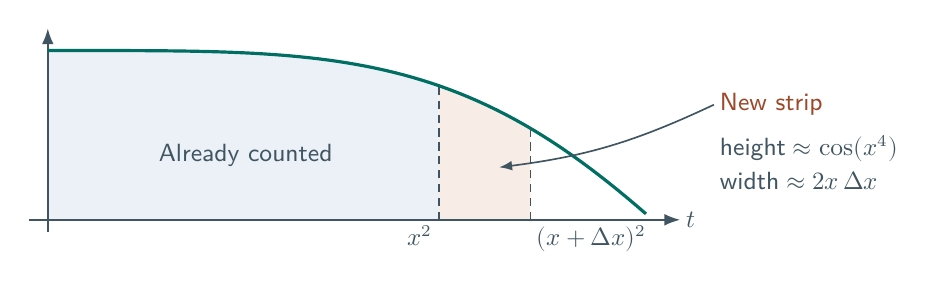
\begin{tikzpicture}[x=6.13cm,y=2.15cm]
\fill[BlueTint] (0,0)--plot[domain=0:.81,samples=35] (\x,{cos((\x*\x) r)})--(.81,0)--cycle;
\fill[RustTint] (.81,0)--plot[domain=.81:1,samples=25] (\x,{cos((\x*\x) r)})--(1,0)--cycle;
\draw[axis] (-.04,0)--(1.31,0) node[lab,right] {\(t\)};
\draw[axis] (0,-.07)--(0,1.13);
\draw[fcurve,domain=0:1.24,samples=65] plot (\x,{cos((\x*\x) r)});
\draw[guide] (.81,0)--(.81,.791) (1,0)--(1,.5403);
\node[lab] at (.41,.38) {Already counted};
\node[lab,right,text=Rust] (extra) at (1.38,.68) {New strip};
\draw[lead] (extra.west) to[bend left=9] (.935,.31);
\node[lab,right] at (1.38,.42) {\(\text{height}\approx\cos(x^4)\)};
\node[lab,right] at (1.38,.23) {\(\text{width}\approx2x\,\Delta x\)};
\node[lab,below left] at (.81,0) {\(x^2\)};
\node[lab,below right] at (1,0) {\((x+\Delta x)^2\)};
\end{tikzpicture}
}{The curve is \(f(t)=\cos(t^2)\), shown at \(x=0.9\) with an exaggerated positive step. Dividing the strip's area by \(\Delta x\) gives approximately its height times the speed of the edge.}

\sectiontitle{Why this problem earned its place}
The question is deliberately set up so that hunting for an elementary antiderivative is not a useful plan. You don't need one. When the boundary moves a little, the previously accumulated area cancels in the difference between the two totals. The question concerns only the new strip. This makes a big theorem feel like a natural answer to a visible problem.

\sectiontitle{Where it sits in calculus}
For continuous \(f\), the rate of change of \(G(u)=\int_0^u f(t)\,dt\) is \(G'(u)=f(u)\). This is one direction of the Fundamental Theorem. The other direction lets you evaluate a definite integral from an antiderivative at the two endpoints. Here \(u=x^2\), so the chain rule also supplies \(u'=2x\). The result joins the accumulation in 06 to the reasoning about coupled rates in 03.

\sectiontitle{What to notice in the Python}
One route evaluates \(\cos(x^4)\,2x\) directly. The independent numerical route estimates areas at two nearby inputs, then differences them. The match is a check. The direct formula comes from seeing why the nearby area, not the old total, determines the derivative.

\bridge{Chain rule + sums}{Rates and totals fit}{Variable boundaries}
\tryit{A tank receives a variable inflow \(q(t)\). A display shows the amount received by clock time \(3x\). How fast does the displayed total change with respect to \(x\)?}
\folio{The Fundamental Theorem}

\chapter{Blue}{08}{What if the interval never ends?}{ACCUMULATION \quad IMPROPER INTEGRALS}
\openq{If water keeps entering the tank forever but the flow weakens, does the total have to be infinite?}
\plate{
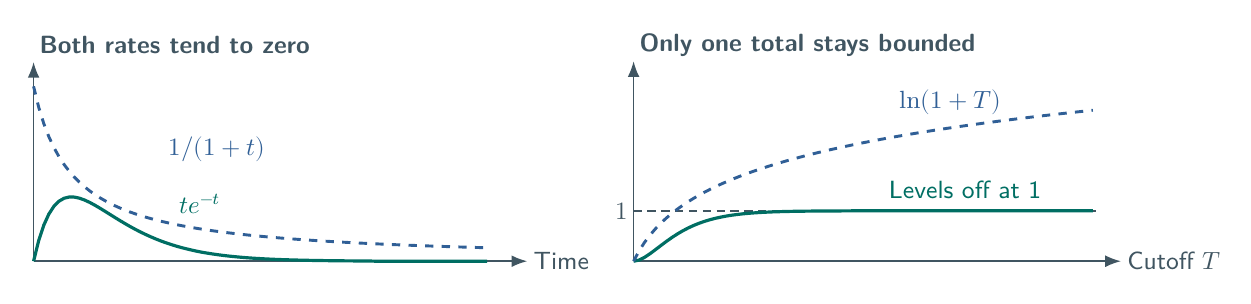
\begin{tikzpicture}[x=1cm,y=1cm]
\begin{scope}
\node[lab,anchor=west,font=\sffamily\bfseries\small] at (0,2.75) {Both rates tend to zero};
\draw[axis] (0,0)--(6.27,0) node[lab,right] {Time};
\draw[axis] (0,0)--(0,2.53);
\draw[fcurve,domain=0:12,samples=90] plot ({\x*.48},{2.22*\x*exp(-\x)});
\draw[bcurve,dashed,domain=0:12,samples=90] plot ({\x*.48},{2.22/(1+\x)});
\node[lab,text=Blue] at (2.33,1.42) {\(1/(1+t)\)};
\node[lab,text=Teal] at (2.12,.73) {\(t e^{-t}\)};
\end{scope}
\begin{scope}[shift={(7.62,0)}]
\node[lab,anchor=west,font=\sffamily\bfseries\small] at (0,2.75) {Only one total stays bounded};
\draw[axis] (0,0)--(6.19,0) node[lab,right] {Cutoff \(T\)};
\draw[axis] (0,0)--(0,2.54);
\draw[guide] (0,.64)--(5.87,.64);
\draw[fcurve,domain=0:19,samples=85] plot ({\x*.307},{.64*(1-(1+\x)*exp(-\x))});
\draw[bcurve,dashed,domain=0:19,samples=85] plot ({\x*.307},{.64*ln(1+\x)});
\node[lab,left] at (0,.64) {\(1\)};
\node[lab,text=Blue] at (4.02,2.02) {\(\ln(1+T)\)};
\node[lab,text=Teal] at (4.21,.90) {Levels off at 1};
\end{scope}
\end{tikzpicture}
}{The left graph depicts instantaneous rate. The right graph depicts accumulated amount so far. Both rates vanish, but the slower-decaying one keeps adding enough to make the total grow without bound.}

\sectiontitle{Why this problem earned its place}
It gives a direct counterexample to a tempting intuition: if the input becomes negligible, surely the total will settle. The contrast between exponential decay and \(1/(1+t)\) makes that reasoning fail in plain sight. You learn to ask not only whether the rate shrinks, but whether it shrinks fast enough.

\sectiontitle{Where it sits in calculus}
A definite integral up to a finite cutoff \(T\) is ordinary accumulation. An improper integral asks if those finite totals approach a finite limit as \(T\) grows. Here integration by parts supplies \(1-(T+1)e^{-T}\), and the limit supplies the total \(1\) liter. That separation matters. The same question appears when checking whether a probability density has finite mass or an infinite series has a finite sum.

\sectiontitle{What to notice in the Python}
The program compares midpoint sums with the exact formula at several finite cutoffs. It also plots the slow total on a logarithmic time axis to show growth over a wider range. No simulation needs to run forever, and no finite run by itself proves convergence.

\bridge{Definite integral + limit}{Convergent totals}{Series tests}
\tryit{Compare the tails of the two rates \(1/t\) and \(1/t^2\) for \(t\geq1\). Both tend to zero. Which has a finite accumulated total? Check using finite cutoffs first.}
\folio{Accumulation}

\chapter{Rust}{09}{Can a rate law predict?}{MODELING \quad DIFFERENTIAL EQUATIONS}
\openq{We don't know the entire cooling curve. Can one rule about change and one follow-up reading give us a useful prediction?}
\plate{
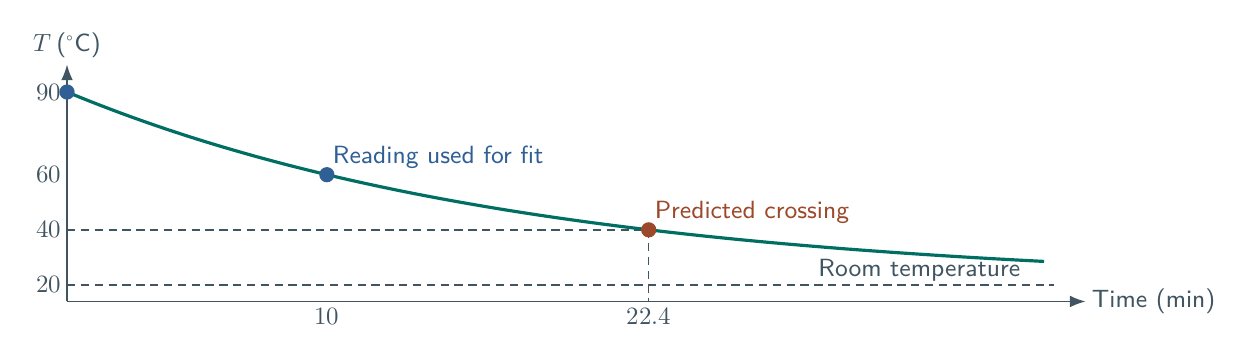
\begin{tikzpicture}[x=.33cm,y=.035cm]
\draw[axis] (0,14)--(39.2,14) node[lab,right] {Time (min)};
\draw[axis] (0,14)--(0,100) node[lab,above] {\(T\) (\({}^{\circ}\)C)};
\draw[guide] (0,20)--(38,20);
\draw[guide] (0,40)--(22.386,40)--(22.386,14);
\draw[fcurve,domain=0:37.6,samples=90] plot (\x,{20+70*exp(-.05596158*\x)});
\fill[Blue] (0,90) circle (2.75pt) (10,60) circle (2.75pt);
\fill[Rust] (22.386,40) circle (2.75pt);
\node[lab,left] at (0,90) {\(90\)};
\node[lab,left] at (0,60) {\(60\)};
\node[lab,left] at (0,40) {\(40\)};
\node[lab,left] at (0,20) {\(20\)};
\node[lab,below] at (10,14) {\(10\)};
\node[lab,below] at (22.386,14) {\(22.4\)};
\node[lab,text=Blue,above right] at (10,60) {Reading used for fit};
\node[lab,text=Rust,above right] at (22.386,40) {Predicted crossing};
\node[lab] at (32.8,25.5) {Room temperature};
\end{tikzpicture}
}{The supplied initial temperature sets the starting point. The 10-minute reading fixes a parameter. The crossing near 22.4 minutes is a model prediction, not another measurement.}

\sectiontitle{Why this problem earned its place}
In the cart problems, you are handed the motion or rate to analyze. Here you don't have the function you want. Instead, you hypothesize a rule about how it changes, use a reading to fit the rule, and get a prediction that a later observation could contradict. It's a small, complete example of using calculus to construct and test a model.

\sectiontitle{Where it sits in calculus}
With \(E=T-T_{\mathrm{room}}\), the rule is \(E'=-kE\). The derivative measures the rate, and the equation ties that rate to the current state. A starting condition picks a trajectory once \(k\) is specified. The follow-up observation estimates \(k\). This pattern recurs in circuits, population models, and feedback systems, even when the equations must be solved numerically.

\sectiontitle{What to notice in the Python}
The exponential solution and the Euler loop express the same rule differently. The loop updates the state by adding rate times elapsed time. Reducing the step size improves agreement with the exact model in this example. Agreement between two implementations does not test whether actual coffee behaves that way.

\bridge{Instantaneous rate}{A rule for the state}{Numerical simulation}
\tryit{The cup is moved to a warmer room after 10 minutes. What should the model carry forward without a jump? What part of the rule must change?}
\folio{Modeling}

\chapter{Rust}{10}{When can you stop adding terms?}{INFINITE PROCESSES \quad SERIES AND ERROR}
\openq{It isn't enough to know an answer is getting closer. How can you certify the first step at which it is close enough?}
\plate{
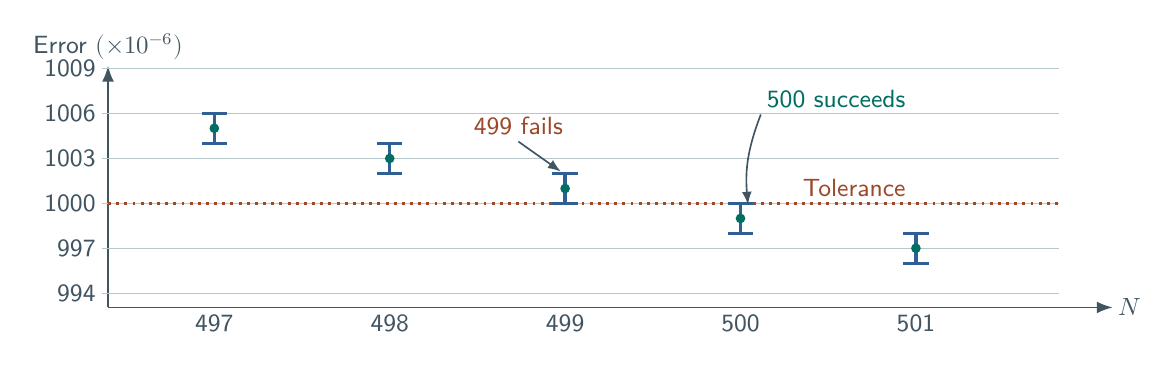
\begin{tikzpicture}[x=1.35cm,y=.19cm]
\draw[axis] (0,.05)--(9.45,.05) node[lab,right] {\(N\)};
\draw[axis] (0,.05)--(0,16.2) node[lab,above] {Error \((\times 10^{-6})\)};
\foreach \y/\val in {1/994,4/997,7/1000,10/1003,13/1006,16/1009}{
 \draw[draw=Faint,thin] (-.06,\y)--(8.95,\y);
 \node[lab,left] at (-.06,\y) {\val};}
\draw[rcurve,dash pattern=on 1.05pt off 1.9pt] (0,7)--(8.95,7);
\node[lab,text=Rust,anchor=west] at (6.48,8.03) {Tolerance};
\foreach \xx/\N/\a/\b/\o in {1/497/11.01606/13.02812/12.02411,2.65/498/9.00401/11.00802/10.00802,4.3/499/7.00000/8.99601/8.00000,5.95/500/5.00399/6.99205/6.00000,7.6/501/3.01594/4.99609/4.00798}{
 \draw[bcurve,line width=1.2pt] (\xx,\a)--(\xx,\b);
 \draw[bcurve] (\xx-.12,\a)--(\xx+.12,\a) (\xx-.12,\b)--(\xx+.12,\b);
 \fill[Teal] (\xx,\o) circle (1.75pt);
 \node[lab,below] at (\xx,0) {\N};}
\node[lab,text=Rust] (fail) at (3.86,12.15) {499 fails};
\draw[lead] (fail.south) -- (4.26,9.13);
\node[lab,text=Teal] (success) at (6.85,13.95) {500 succeeds};
\draw[lead] (success.south west) to[bend right=13] (6.02,6.91);
\end{tikzpicture}
}{Blue bars show bounds on the true error. Dots are numerical estimates. At 499 the error is strictly above its lower bound, which equals the tolerance. At 500 the upper bound is below the tolerance. The vertical scale is magnified.}

\sectiontitle{Why this problem earned its place}
It exposes the difference between a theorem that gives a usable answer and a sharper argument that gives the \emph{first} usable answer. The standard alternating-series bound certifies 999 terms. Keeping the finite geometric remainder and bounding its integral certifies 500 terms and rules out 499. Those are compatible answers to different questions about the same series.

\sectiontitle{Where it sits in calculus}
A series is a limit of finite partial sums. Here the exact error is the positive integral \(\int_0^1 x^N/(1+x)\,dx\). It shrinks as \(N\) increases, which is why ruling out 499 rules out all smaller counts. This problem pulls together limits (01), error bounds (05), and definite integration (06). It points toward algorithm design, where a guarantee about the remaining error can tell software when to stop.

\sectiontitle{What to notice in the Python}
The script uses exact fractions to compare the bounds with \(1/1000\). The plotted dots are computed from floating-point partial sums and a reference value of \(\ln 2\). Near the threshold, the rational comparisons carry the proof, regardless of how the dots round on the screen.

\bridge{Finite sum + integral}{Certified stopping}{Reliable algorithms}
\tryit{If a more expensive method guarantees the same tolerance with fewer terms, what else would you need to know before calling it the better algorithm?}
\folio{Infinite processes}

\clearpage\colorlet{Accent}{Blue}\pdfbookmark[0]{The decision guide}{toolkit}
\tagline{PUT IT TO WORK \quad / \quad A DECISION GUIDE}
\vspace{4pt}\headline{Which tool do I need?}
\vspace{5pt}
On a test, the chapter title usually tells you which method to use. Outside a textbook, the first task is figuring out what kind of answer the situation calls for. Read down the left column until you recognize what you are trying to find.

\vspace{7pt}
{\setlength{\tabcolsep}{7pt}\renewcommand\arraystretch{1.44}
\begin{tabularx}{\linewidth}{@{}>{\raggedright\arraybackslash}p{1.65in}>{\raggedright\arraybackslash}p{1.55in}>{\raggedright\arraybackslash}Xr@{}}
\toprule
\smallcap{IF YOU WANT\ldots}&\smallcap{REACH FOR\ldots}&\smallcap{DO NOT OVERLOOK}&\smallcap{NO.}\\
\midrule
What a quantity approaches & A limit & Its value at the point is a separate question. & \chaplink{01}{01}\\
A rate at a particular instant & A derivative & Start with what changes over an interval. & \chaplink{02}{02}\\
The rate of a connected quantity & The chain rule & Keep the time dependence until after differentiating. & \chaplink{03}{03}\\
The best allowable choice & Constrained optimization & Endpoints, feasibility, and other candidates. & \chaplink{04}{04}\\
A nearby value with stated accuracy & A Taylor approximation & The remainder is what backs up the claim. & \chaplink{05}{05}\\
A total from a changing rate & A definite integral & Net and gross totals may answer different questions. & \chaplink{06}{06}\\
The rate at which a total grows & The Fundamental Theorem & If the boundary moves, multiply by its speed. & \chaplink{07}{07}\\
A total over an unbounded interval & An improper integral & A rate approaching zero does not prove convergence. & \chaplink{08}{08}\\
A trajectory from a rule about change & A differential equation & Fitting data and testing a prediction are different. & \chaplink{09}{09}\\
A defensible place to stop & A remainder bound & A guarantee can be valid without being sharp. & \chaplink{10}{10}\\
\bottomrule
\end{tabularx}}
\vspace{14pt}

\sectiontitle{What ten problems cannot cover}
This is a map of single-variable calculus, not a full syllabus. It's deliberately light on symbolic differentiation and integration drills, and it does not survey multivariable or vector calculus. It gives you the questions those larger courses build on: What changes locally? What accumulates? What does the model predict? How good is the answer?

\folio{Decision guide}

\clearpage\colorlet{Accent}{Teal}\pdfbookmark[0]{Transfer test notes}{key}
\tagline{PUT IT TO WORK \quad / \quad TRANSFER TEST NOTES}
\vspace{4pt}\headline{Same idea, different setting}
\vspace{4pt}
Try the questions first. These brief answers identify what should carry over when the original cart, ladder, box, or coffee cup is gone.

\vspace{6pt}
\newcommand{\key}[3]{\par\vspace{5pt}\noindent
\begin{minipage}{\linewidth}\raggedright
{\sffamily\bfseries\color{Teal}\chaplink{#1}{#1}\enspace #2.}\enspace#3
\end{minipage}\par}
\key{01}{The size matters}{\(\lvert x^2\cos(1/x^3)\rvert\le x^2\), so the limit is zero. How fast the cosine cycles does not affect the bound.}
\key{02}{The sensor estimate}{Use readings on both sides of the middle time. Divide the difference in positions by the elapsed time between them. Compare estimates for several intervals or against a reference. Shorter intervals can expose noise or limited resolution.}
\key{03}{The widening tank}{The inflow required is \(dV/dt=A(h)\,dh/dt\), where \(A(h)\) is the area of the water surface at height \(h\). If that area increases, holding the rise speed fixed requires more inflow.}
\key{04}{The depth cap}{The allowable interval is now \([0,2]\). Both original derivative roots lie outside it, and \(V'(0)>0\), so the volume increases across the interval. The best allowable cut is 2 inches.}
\key{05}{Rounding versus the bound}{The value is between \(0.904833\) and \(0.905\). Every number there rounds to \(0.905\) at three decimal places. That interval alone does not determine the fourth decimal place.}
\key{06}{The battery log}{Sum \(I\,\Delta t\) for net change in charge and \(\lvert I\rvert\,\Delta t\) for total charge moved, using representative currents and actual interval widths. Amperes times seconds gives coulombs.}
\key{07}{The accelerated clock}{The accumulated amount as a function of \(x\) is \(\int_0^{3x}q(t)\,dt\), so its derivative is \(3q(3x)\) wherever \(q\) is continuous at the edge.}
\key{08}{Two decaying tails}{From \(1\) to \(T\), the totals are \(\ln T\) and \(1-1/T\), respectively. Only the second stays finite in the limit.}
\key{09}{The room changes}{Carry the coffee's temperature forward continuously at the move. Replace the ambient temperature in the rate law. If airflow or other conditions change, the fitted \(k\) might also change.}
\key{10}{The cheaper answer}{Count total work, not just terms. A method with fewer terms may spend more time or memory per term. Compare cost and numerical reliability at the same guaranteed accuracy.}
\folio{Transfer test notes}

\end{document}
